\subsection{RIPS}
RIPS was used for static analysis of PHP code as the first step in finding vulnerablities in the application.
\subsubsection{Online Banking }
Online Banking showed 193 issues. Refer \ref{fig:rips_overview}. The tool reported the following issues:
\begin{itemize}
    \item Command Execution - Refer \ref{fig:rips_command_execution}.
    \item File Inclusion - Refer \ref{fig:rips_file_inclusion}.
    \item File Manipulation - Refer \ref{fig:rips_file_manipulation}.
    \item Reflection Injection - Refer \ref{fig:rips_reflection_injection}.
    \item Session Fixation - Refer \ref{fig:rips_session_fixation}.
    \item XSS - Refer \ref{fig:rips_xss}.
    \item SQL Injection - Refer \ref{fig:rips_sql_injection}.
\end{itemize}
57\% of the issues were found to be false positives which was also confirmed by black box testing and manual code inspection.

\subsubsection{SecureBank}
SecureBank showed 331 issues. This is reasonable owing to the number of files. Refer \ref{fig:rips_overview_secure_bank}. The tool reported the following issues:
\begin{itemize}
    \item Command Execution - Refer \ref{fig:rips_command_execution_secure_bank}.
    \item Code Execution - Refer \ref{fig:rips_code_execution_secure_bank}.
    \item File Manipulation - Refer \ref{fig:rips_file_manipulation_secure_bank}.
    \item Reflection Injection - Refer \ref{fig:rips_reflection_injection_secure_bank}.
    \item HTTP Response Splitting - Refer \ref{fig:rips_http_resp_splitting_secure_bank}.
    \item XSS. Refer - \ref{fig:rips_xss_secure_bank}.
\end{itemize}

All the above issues were found to be false positives which was also confirmed by black box testing and manual code inspection.

\begin{figure}[ht]
	\centering
	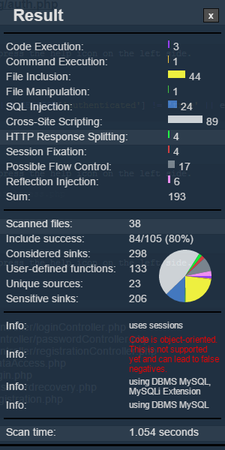
\includegraphics[width=.6\linewidth]{figures/rips_overview.png}
	\caption{Overview of RIPS scan for Online Banking}
	\label{fig:rips_overview}
\end{figure}

\begin{figure}[ht]
	\centering
	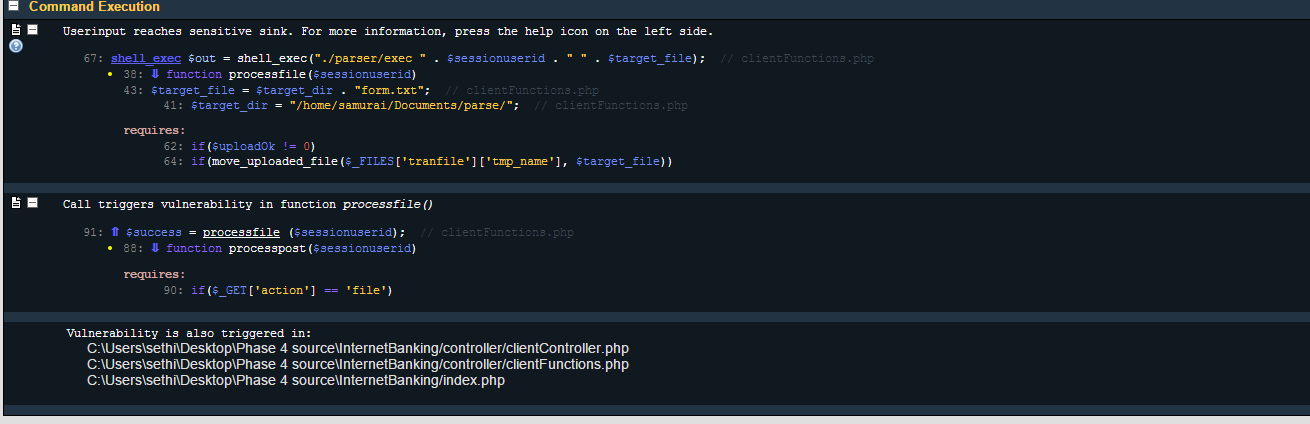
\includegraphics[width=.8\linewidth]{figures/rips_command_execution.png}
	\caption{RIPS: Command Execution vulnerability reported for Online Banking}
	\label{fig:rips_command_execution}
\end{figure}

\begin{figure}[ht]
	\centering
	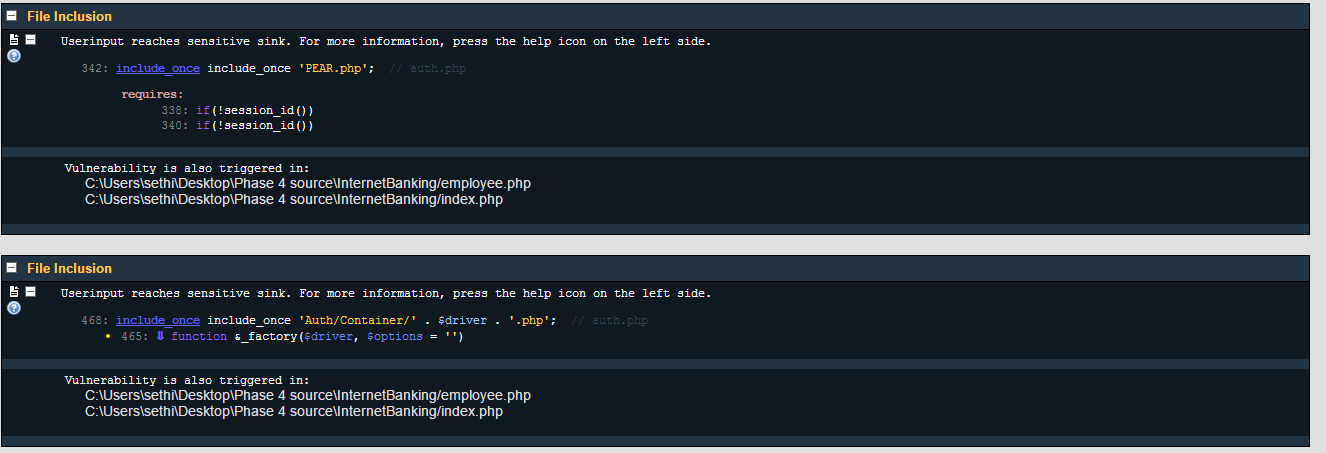
\includegraphics[width=.8\linewidth]{figures/rips_file_inclusion.png}
	\caption{RIPS: File Inclusion vulnerability reported for Online Banking}
	\label{fig:rips_file_inclusion}
\end{figure}

\begin{figure}[ht]
	\centering
	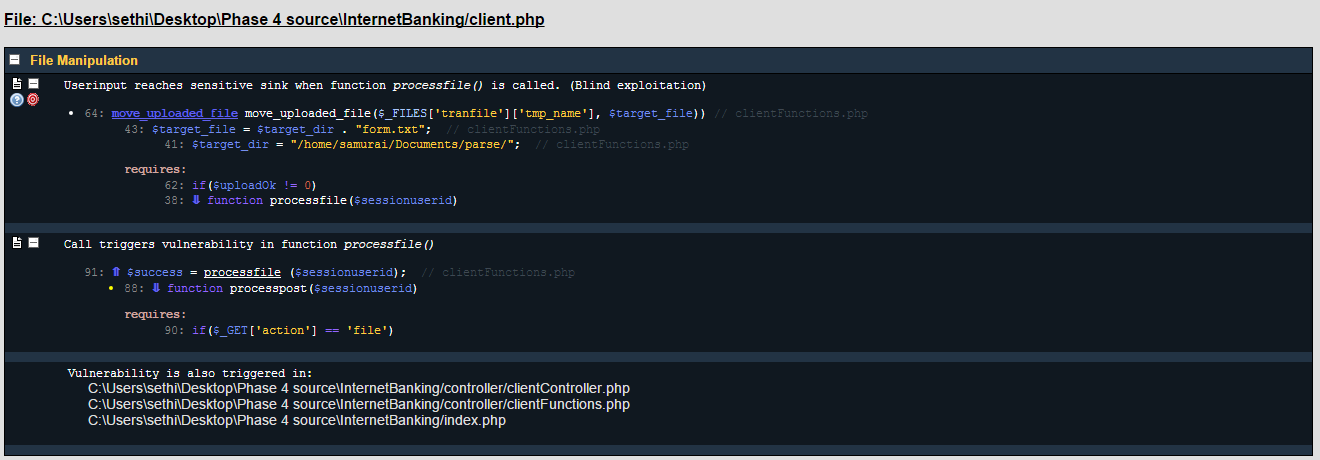
\includegraphics[width=.8\linewidth]{figures/rips_file_manipulation.png}
	\caption{RIPS: File Manipulation vulnerability reported for Online Banking}
	\label{fig:rips_file_manipulation}
\end{figure}

\begin{figure}[ht]
	\centering
	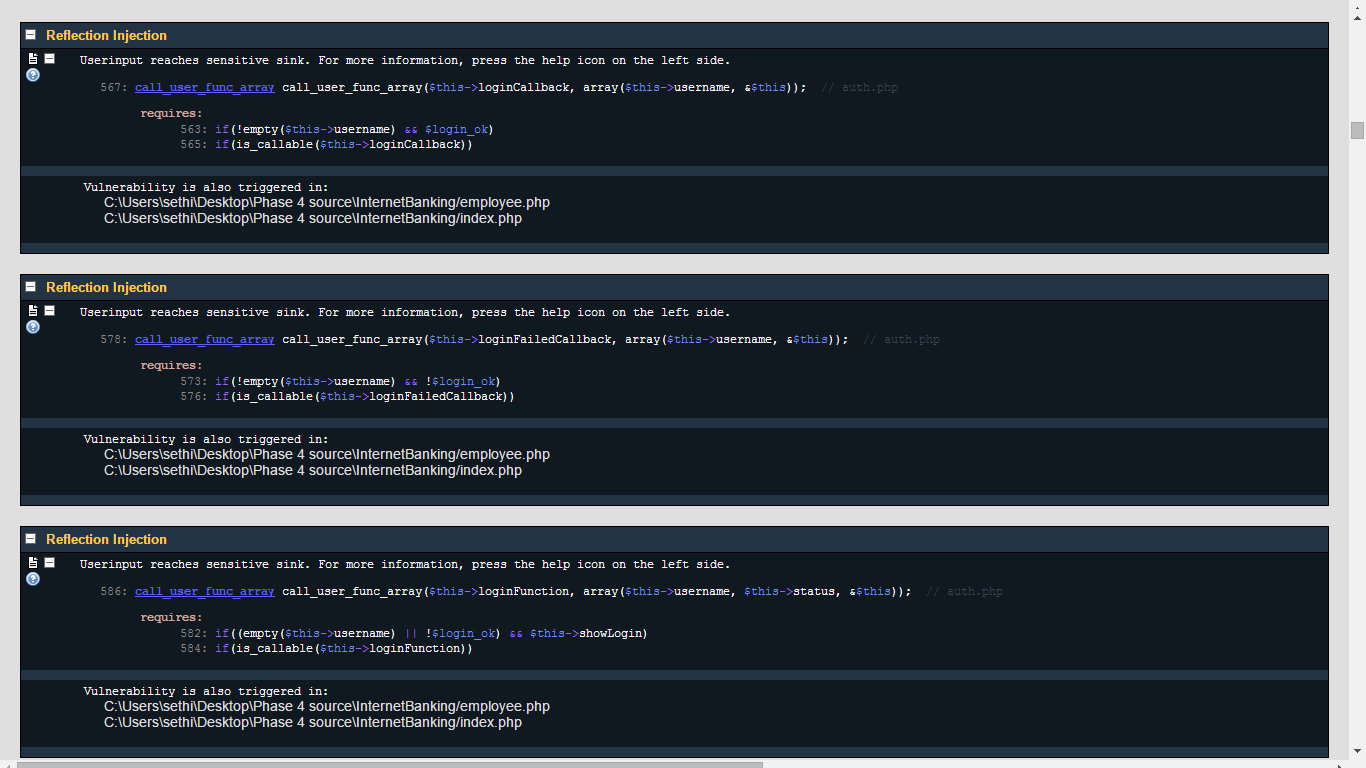
\includegraphics[width=.8\linewidth]{figures/rips_reflection_injection.png}
	\caption{RIPS: Reflection Injection vulnerability reported for Online Banking}
	\label{fig:rips_reflection_injection}
\end{figure}

\begin{figure}[ht]
	\centering
	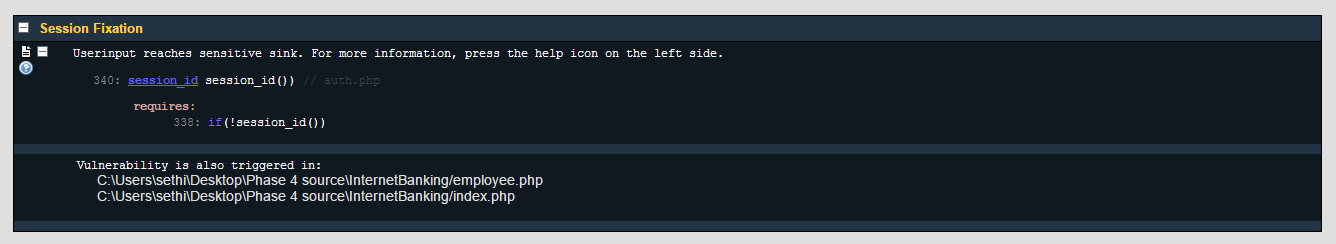
\includegraphics[width=.8\linewidth]{figures/rips_session_fixation.png}
	\caption{RIPS: Session Fixation vulnerability reported for Online Banking}
	\label{fig:rips_session_fixation}
\end{figure}


\begin{figure}[ht]
	\centering
	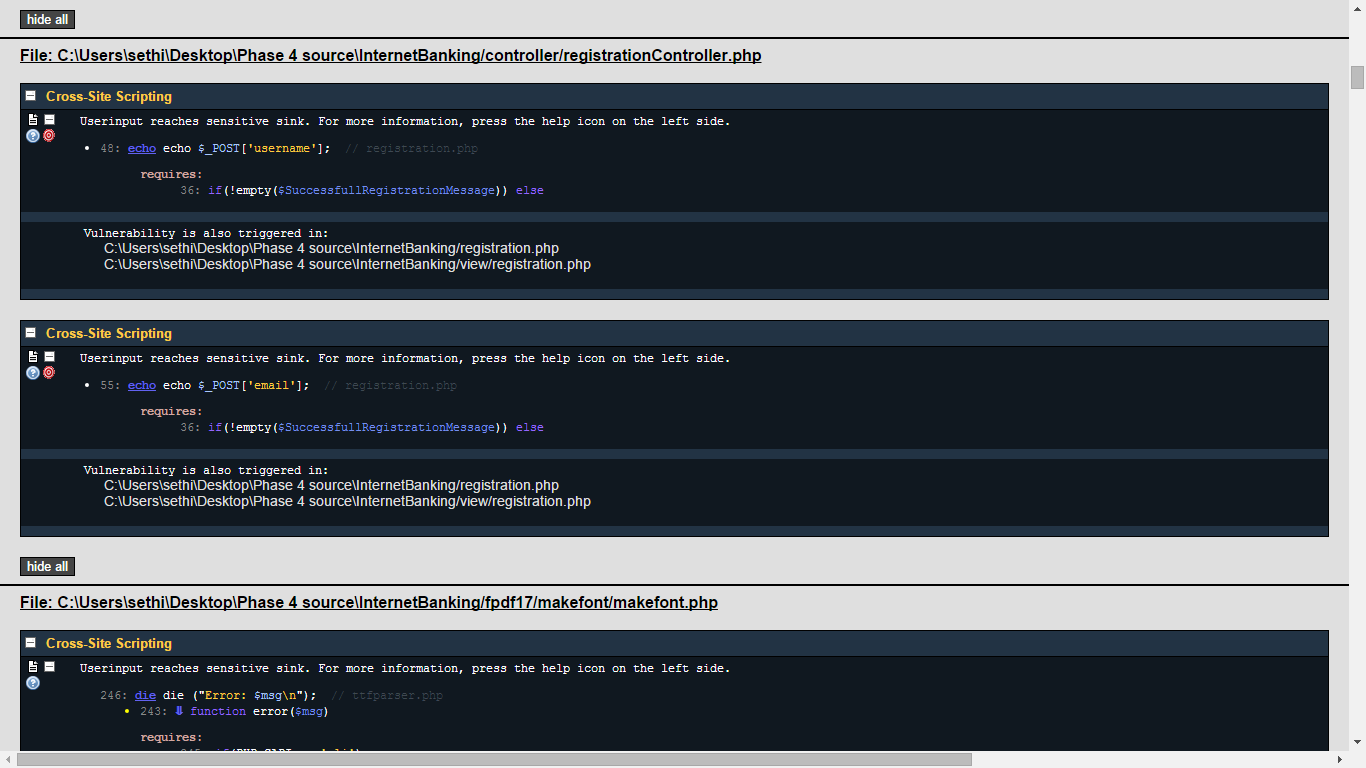
\includegraphics[width=.8\linewidth]{figures/rips_xss.png}
	\caption{RIPS: Cross Site Scripting vulnerability reported for Online Banking}
	\label{fig:rips_xss}
\end{figure}


\begin{figure}[ht]
	\centering
	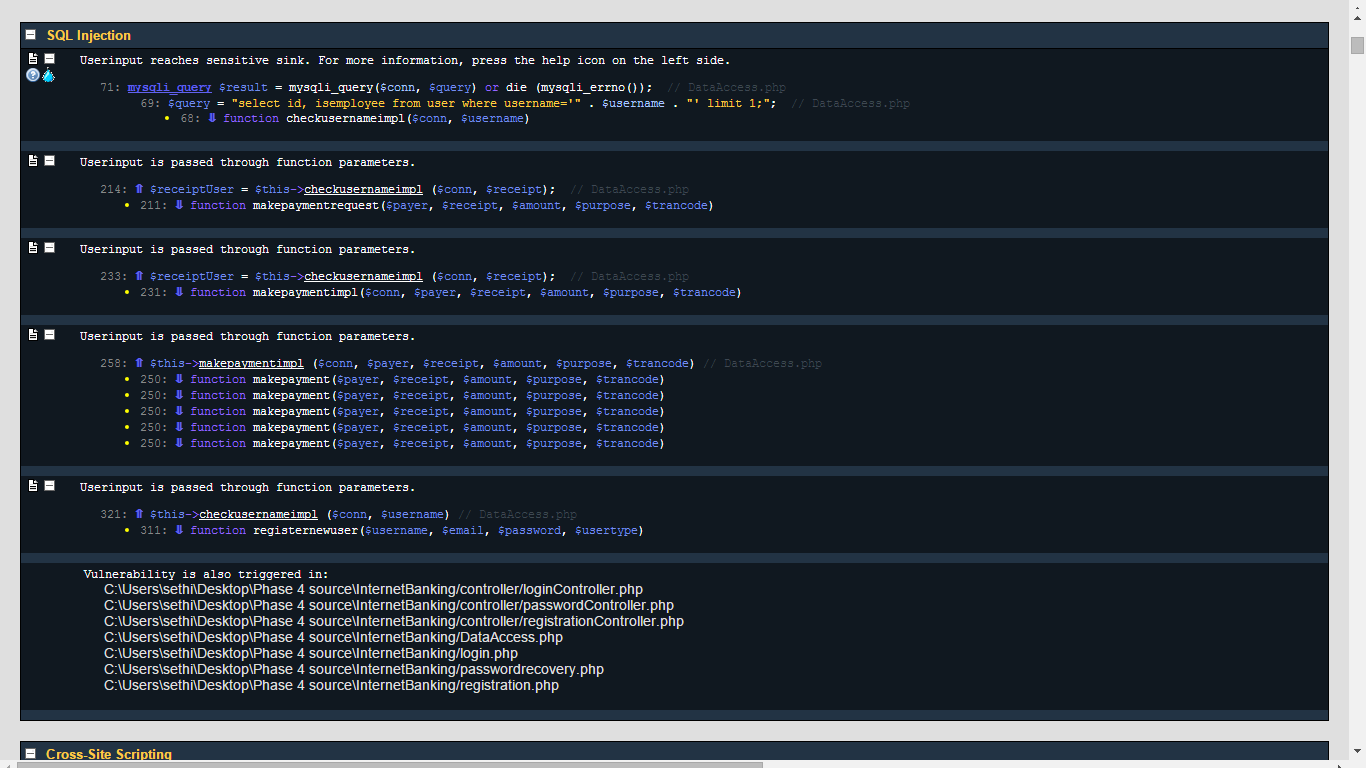
\includegraphics[width=.8\linewidth]{figures/rips_sql_injection.png}
	\caption{RIPS: SQL Injection vulnerability reported for Online Banking}
	\label{fig:rips_sql_injection}
\end{figure}



\begin{figure}[ht]
	\centering
	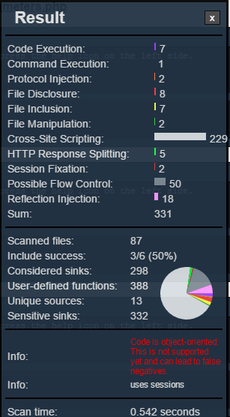
\includegraphics[width=.6\linewidth]{figures/rips_overview_secure_bank.png}
	\caption{Overview of RIPS scan for SecureBank}
	\label{fig:rips_overview_secure_bank}
\end{figure}

\begin{figure}[ht]
	\centering
	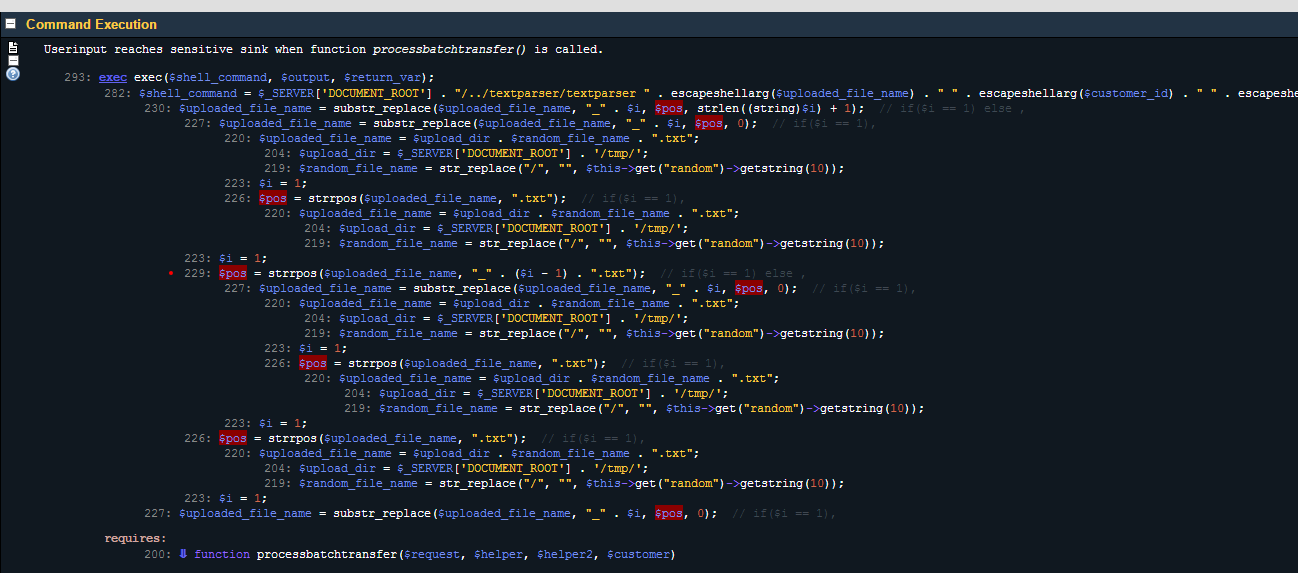
\includegraphics[width=.8\linewidth]{figures/rips_command_execution_secure_bank.png}
	\caption{RIPS: Command Execution vulnerability reported for SecureBank}
	\label{fig:rips_command_execution_secure_bank}
\end{figure}

\begin{figure}[ht]
	\centering
	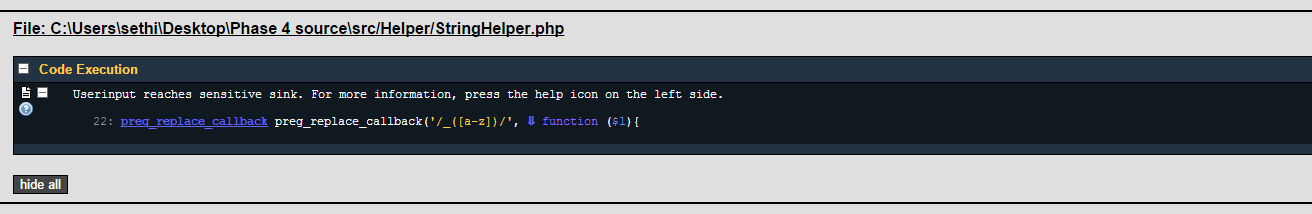
\includegraphics[width=.8\linewidth]{figures/rips_code_execution_secure_bank.png}
	\caption{RIPS: Code Execution vulnerability reported for SecureBank}
	\label{fig:rips_code_execution_secure_bank}
\end{figure}

\begin{figure}[ht]
	\centering
	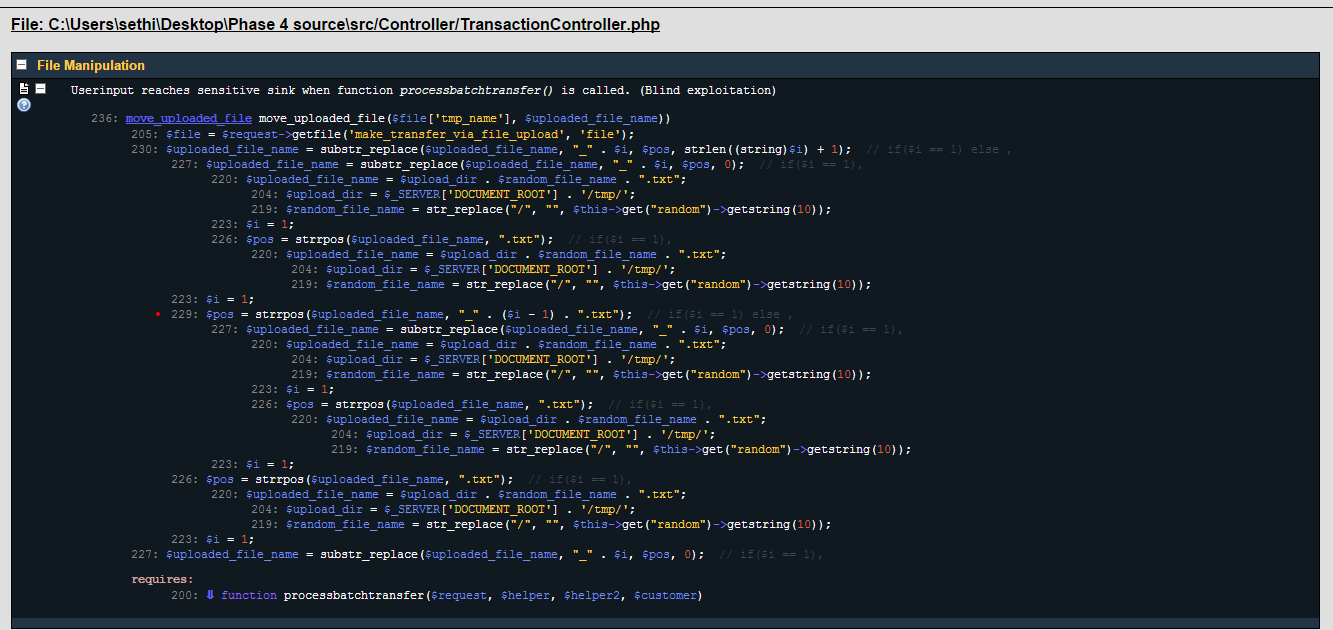
\includegraphics[width=.8\linewidth]{figures/rips_file_manipulation_secure_bank.png}
	\caption{RIPS: File Manipulation vulnerability reported for SecureBank}
	\label{fig:rips_file_manipulation_secure_bank}
\end{figure}

\begin{figure}[ht]
	\centering
	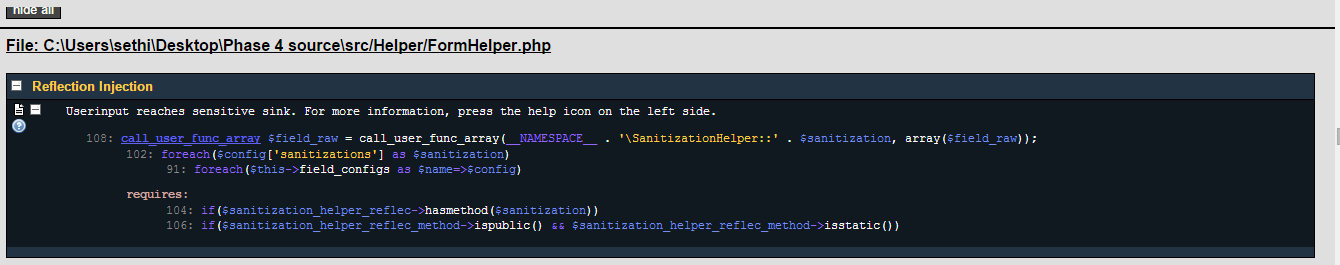
\includegraphics[width=.8\linewidth]{figures/rips_reflection_injection_secure_bank.png}
	\caption{RIPS: Reflection Injection vulnerability reported for SecureBank}
	\label{fig:rips_reflection_injection_secure_bank}
\end{figure}

\begin{figure}[ht]
	\centering
	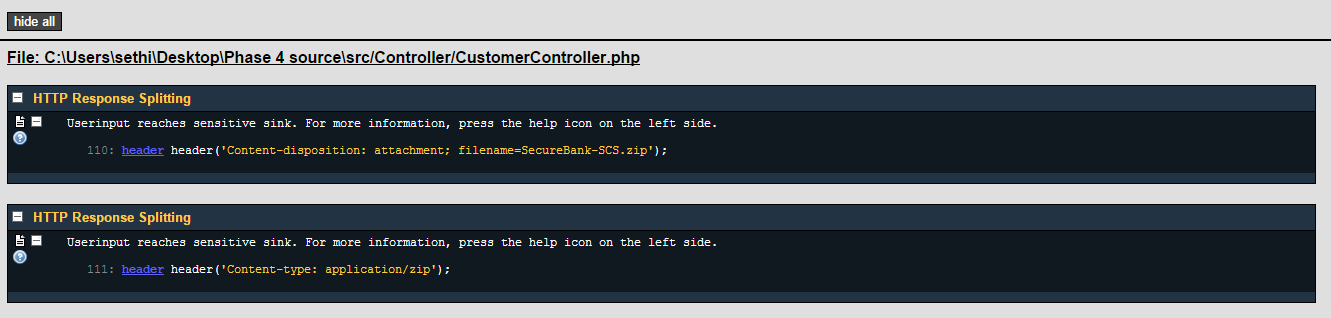
\includegraphics[width=.8\linewidth]{figures/rips_http_resp_splitting_secure_bank.png}
	\caption{RIPS: HTTP Response Splitting vulnerability reported for SecureBank}
	\label{fig:rips_http_resp_splitting_secure_bank}
\end{figure}


\begin{figure}[ht]
	\centering
	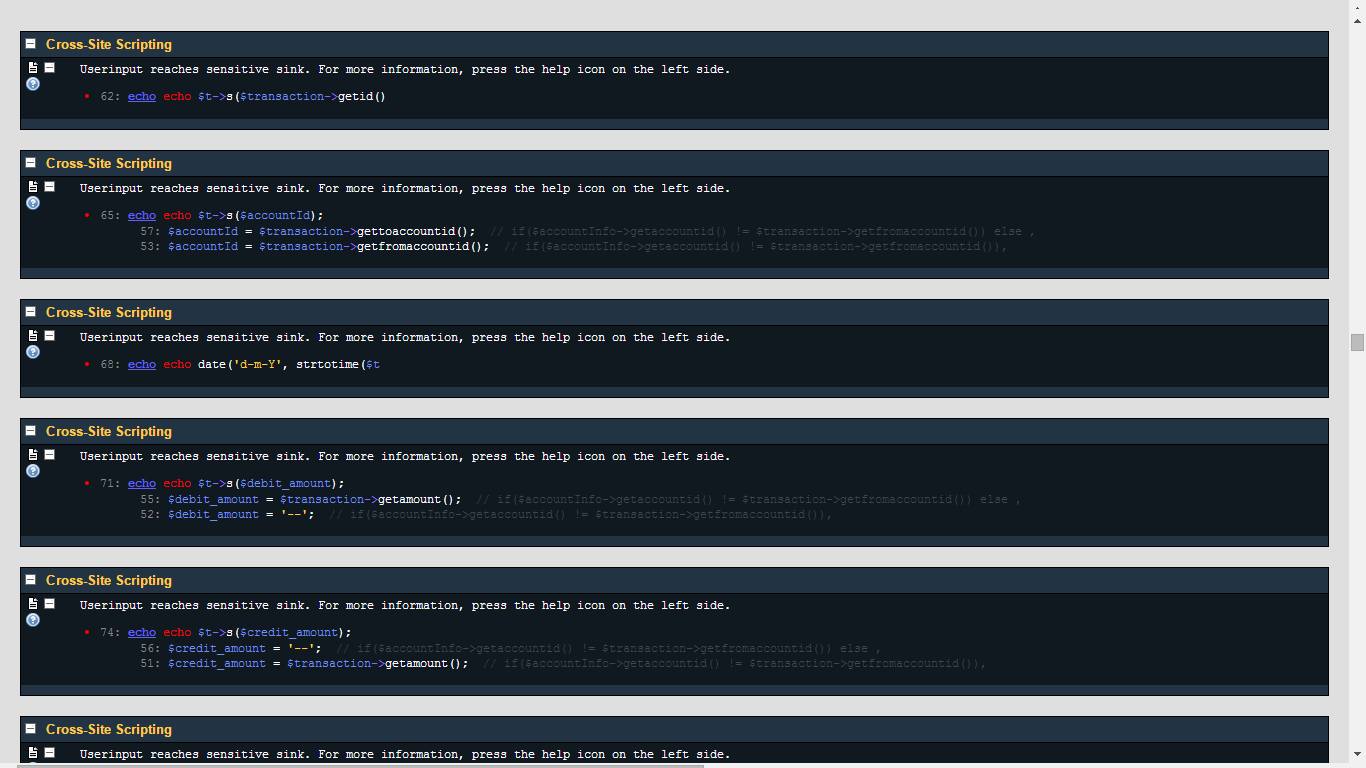
\includegraphics[width=.8\linewidth]{figures/rips_xss_secure_bank.png}
	\caption{RIPS: Cross Site Scripting vulnerability reported for SecureBank}
	\label{fig:rips_xss_secure_bank}
\end{figure}